\documentclass[11pt,a4paper]{article}

%======================================================================
% Title, author and date
%======================================================================

\title{
	Projektdokumentation\\
	Transportüberwachungssystem Roadrunner
}
\author{
	Franziskus Domig, B.Sc.\\
		\and
	Stefan Gassner, B.Sc.\\
		\and
	Wolfgang Halbeisen, B.Sc.\\
		\and
	Matthias Schmid, B.Sc.\\	
}
\date{\today}

%======================================================================
% Packages
%======================================================================

%%%%%%%%%%%%%%%%%%%%%%%%%%%%%%%%%%%%%%%%%%%%%%%%%%%%%%%%%%%%%%%%%%%%%
% Packages

% für \hyphenation mit Umlauten
\usepackage[T1]{fontenc}
\usepackage[utf8]{inputenc}
\usepackage[ngerman,english]{babel}

% Times-Roman-Schrift (auch für mathematische Formeln)
\usepackage{mathptmx} 

% comments
\usepackage{verbatim} 

% Zum Setzen von URLs
\usepackage{color}
\usepackage{alltt}
\definecolor{darkred}{rgb}{.25,0,0}
\definecolor{darkgreen}{rgb}{0,.2,0}
\definecolor{darkmagenta}{rgb}{.2,0,.2}
\definecolor{darkcyan}{rgb}{0,.15,.15}

\usepackage[plainpages=false,bookmarks=true,bookmarksopen=true,colorlinks=true,
  linkcolor=darkred,citecolor=darkgreen,filecolor=darkmagenta,
  menucolor=darkred,urlcolor=darkcyan]{hyperref}

% Zeilenabstand
\renewcommand{\baselinestretch}{1.5}

% anhang
\usepackage[toc,page]{appendix}

% pdflatex: Bilder in den Formaten .jpeg, .png und .pdf
% latex: Bilder im .eps-Format
\usepackage{graphicx}

\usepackage{fancyhdr} % Positionierung der Seitenzahlen
\fancyhead{}
\fancyfoot[C]{\Roman{page}}
\renewcommand{\headrulewidth}{0pt}
\setlength{\headheight}{13.6pt} % behebt headheight Warning

 % behebt headheight Warning
\setlength{\headheight}{13.6pt}

% Korrektes Format für Nummerierung von Abbildungen (figure) und
% Tabellen (table): <Kapitelnummer>.<Abbildungsnummer>
\makeatletter
\@addtoreset{figure}{section}
\renewcommand{\thefigure}{\thesection.\arabic{figure}}
\@addtoreset{table}{section}
\renewcommand{\thetable}{\thesection.\arabic{table}}
\makeatother

% Listings für Sourcecode
\usepackage{listings}
  \usepackage{courier}
 \lstset{
        basicstyle=\footnotesize\ttfamily, % Standardschrift
        numbers=left,               % Ort der Zeilennummern
        numberstyle=\tiny,          % Stil der Zeilennummern
        %stepnumber=2,               % Abstand zwischen den Zeilennummern
        numbersep=5pt,              % Abstand der Nummern zum Text
        tabsize=2,                  % Groesse von Tabs
        extendedchars=true,         %
        breaklines=true,            % Zeilen werden Umgebrochen
        keywordstyle=\color{red},
        frame=b,         
        keywordstyle=[1]{\color{DarkSkyBlue}},    % Stil der Keywords
        keywordstyle=[2]{\color{DarkScarletRed}},    %
        keywordstyle=[3]{\bfseries},    %
        keywordstyle=[4]{\color{DarkPlum}},    %
        keywordstyle=[5]{\color{SkyBlue}},    %
		stringstyle={\color{Chocolate}},
        showspaces=false,           % Leerzeichen anzeigen ?
        showtabs=false,             % Tabs anzeigen ?
        xleftmargin=17pt,
        framexleftmargin=17pt,
        framexrightmargin=5pt,
        framexbottommargin=4pt,
        backgroundcolor=\color{Aluminium1},
        showstringspaces=false,      % Leerzeichen in Strings anzeigen ?
		%language=php
		morekeywords=[1]{Interface,return,static,function}
}
    %\DeclareCaptionFont{blue}{\color{blue}} 

  %\captionsetup[lstlisting]{singlelinecheck=false, labelfont={blue}, textfont={blue}}
  \usepackage{caption}
\DeclareCaptionFont{white}{\color{white}}
\DeclareCaptionFormat{listing}{\colorbox[cmyk]{0.43, 0.35, 0.35,0.01}{\parbox{\textwidth}{\hspace{15pt}#1#2#3}}}
\captionsetup[lstlisting]{format=listing,labelfont=white,textfont=white, singlelinecheck=false, margin=0pt, font={bf,footnotesize}}
\renewcommand\lstlistingname{Codeblock}
 

\sloppy % Damit LaTeX nicht so viel über "overfull hbox" u.Ä. meckert

% Ränder
\addtolength{\topmargin}{-16mm}
\setlength{\oddsidemargin}{40mm}
\setlength{\evensidemargin}{40mm}
\addtolength{\oddsidemargin}{-1in}
\addtolength{\evensidemargin}{-1in}
\setlength{\textwidth}{13cm}
\addtolength{\textheight}{34mm}
%______________________________________________________________________

%======================================================================
% PDF settings
%======================================================================

\hypersetup{
	pdfauthor = {
		Franziskus Domig, B.Sc;
		Stefan Gassner, B.Sc.;
		Wolfgang Halbeisen, BSc;
		Matthias Schmid, B.Sc.
	},
	pdftitle = {Projekt Dokumentation Roadrunner},
	pdfkeywords = {Roadrunner, Dokumentation, Transport, Logistik,
		Transportüberwachung},
}

%======================================================================
%      Document
%======================================================================

\begin{document}
	
\selectlanguage{ngerman}

\pagestyle{empty} % Vorerst keine Seitenzahlen
\pagenumbering{alpha} % Unsichtbare alphabetische Nummerierung

\begin{center}

\includegraphics[width=60mm]{files/logo-fhv.png}

\vspace{4cm}
{\large\textbf{Projektdokumentation}}\vspace{.5cm}

{\LARGE Transportüberwachungssystem Roadrunner}

\end{center}

\vspace{13cm}


\begin{tabular}{ll}
	Projektteam: & Franziskus Domig, BSc; Stefan Gassner, BSc;\\
	     	& Wolfgang Halbeisen, BSc; Matthias Schmid, BSc\\
	Bearbeitung: & Dornbirn, im Sommersemester 2011\\
	Betreuer:    & Prof.(FH) DI Wolfgang Auer\\
\end{tabular}

%______________________________________________________________________

\clearpage
\pagestyle{fancy}
\pagenumbering{roman} % Römische Seitenzahlen
\setcounter{page}{1}

\begin{abstract}
	TODO: Hier steht später die Zusammenfassung dieser Arbeit ...
\end{abstract}

% Abstract in english
\begin{otherlanguage}{english}
	\begin{abstract}
		TODO: Here is the later to be written abstract of this paper ...
	\end{abstract}
\end{otherlanguage}

\clearpage
\tableofcontents

\clearpage
\pagenumbering{arabic}
\setcounter{page}{1}

% Geändertes Format für Seitenränder, arabische Seitenzahlen
\fancyfoot[CO]{\thepage}

\section{Motivation}

Ein Transportüberwachungssystem kann aus mehreren Blickwinkeln betrachtet werden.
	In diesem Semesterprojekt ist für die Erstellung eines vollständigen
	Systems zu wenig Zeit vorhanden und somit wird in diesem Projekt der Fokus
	auf die Erstellung einer mobilen Applikation, die Replizierung von Daten auf
	einen Backendserver sowie die Verwaltung des Systems mit einer Webapplikation
	gelegt.
	
Aus oben genannten zeitlichen Gründen wird keine eigene Hardware entwickelt und somit
	die Android Plattform als Host-System für eine mobile Applikation verwendet.
	Zudem werden bis auf eine Ausnahme keine realen Sensoren verwendet sondern
	benötigte Sensoren simuliert.

Dieses Projekt konzentriert sich auf die Entwicklung von Software und wir mit Hilfe
	neuer Technologien, teilweise sogar in Beta-Versionen, implementiert.
	
Auf dem Backendserver wird mit CouchDB ein unkonventioneller Ansatz der
	Datenpersistierung gewählt. Zur Verwaltung von Aufträgen (Lieferungen)
	dient eine Webapplikation.

Als Softwareentwicklungsprozess wird \emph{Test-Driven-Development} gewählt.
	Hierzu wurden nahezu alle entwickelten Komponenten mit \emph{Unit-Tests}
	getestet sowie wenn möglich auf einem \emph{Continuous-Integration}-Server
	bei jeder Änderung automatisiert getestet.

\clearpage
\section{Projektanforderungen}
\label{sec:requirements}

Das Ziel dieses Projekts ist es, ein System zur lückenlosen Transportüberwachung
	zu entwickeln. Hierzu sollen Produkte, welche erst im Rahmen des Projekts zu
	spezifizieren sind, überwacht werden. Es soll nach einem Transport möglich
	sein, eindeutig nachvollziehen zu können, welche Sensor-Daten zu jedem
	Zeitpunkt aufgezeichnet wurden.

Ausgehend von den Anforderungen an ein System für die Transportüberwachung von
	Arzneimitteln in Österreich \cite{PHARMIG07} wird ein System erstellt,
	welches die Temperatur- sowie die Positionsdaten von Lieferungen bzw.
	den darin enthaltenen Paketen aufzeichnet und überwacht.
	
Es soll am Ende dieses Projekts möglich sein, einen einfachen Anwendungsfall
	vollständig	durchzuführen.

\clearpage
\section{Systembeschreibung und -architektur}
\label{sec:system}

In diesem Abschnitt werden die in diesem Projekt verwendeten Technologien
	erläutert. Insbesondere werden die Gründe beschrieben, weswegen diese
	Technologien eingesetzt und anderen vorgezogen werden. Die Vor- sowie
	Nachteile der entsprechenden Technologien werden gegenübergestellt und
	besprochen. Zugleich werden die entsprechenden Technologien auf ihre
	Tauglichkeit in einem real logistischen Szenario geprüft.

\subsection{Mobiles Gerät auf Basis von Android}

Bei diesem Transportüberwachungssystem sollten laut den in
	Kapitel~\ref{sec:requirements} spezifizierten Anforderungen eine lückenlose
	und ständige Überwachung sichergestellt werden. Somit müssen Sensorendaten
	laufend auf ein Backendsystem übertragen werden. Hierzu bietet sich
	die \emph{Android}\footnote{vgl. \url{http://www.android.com/}} Plattform
	als Grundlage für eine mobile Applikation an.
	
Mit Android als Grundlage können gleich mehrere Aspekte abgedeckt werden. Jedes
	Fahrzeug wird mit einem Android Smartphone ausgestattet und ist somit nicht
	nur telefonisch erreichbar sondern gleichzeitig kann die komplette
	Transportüberwachung damit erreicht werden.
	
Mit der entwickelten Applikation lassen sich Gegenstände einladen indem diese
	via Barcode in das System übernommen werden. Ab diesem Zeitpunkt wird dieser
	Gegenstand ständig überwacht und via CouchDB (siehe Abschnitt~\ref{subsec:couchdb})
	mit dem Backensystem synchronisiert. Auf der Webapplikation (siehe
	Abschnitt~\ref{subsec:webapplication}) können die Produkte bzw. die Lieferung,
	welche aus mehreren Produkten bestehen kann nun auf einer Karte	nachverfolgt
	werden sowie die jeweiligen Daten der Temperatursensoren (siehe
	Abschnitt~\ref{subsec:nodejs}) bis zum ausladen überprüft werden.
		
Auch in einem realen Szenario lässt sich Android hervorragend einsetzten. Es ist
	mittlerweile in Version~3.1 (15. Juni 2011) verfügbar und weit verbreitet.
	Die von Google bereitgestellten \emph{Google Apps for Business}\footnote{vgl.
	\url{http://www.google.com/apps/intl/de/business/index.html}} können die
	Smartphones per Fernwartung administriert werden. Dabei können auch
	Applikations-Updates an alle registrierten Smartphones verteilt werden.
	Somit ist auch eine einfache Lösung für das Deployment von neuen Versionen
	gegeben.
	
Im Kapitel~\ref{sec:android} wird die in diesem Projekt erstellte Android Applikation
	beschrieben.

\subsection{Verteiltes Datenbansystem CouchDB}
\label{subsec:couchdb}

Bei einem Transportüberwachungssystem ist die Datensicherung ein
	wichtiger Aspekt. In diesem Kapitel werden unterschiedliche 
	Möglichkeiten der Datenverwaltung betrachtet und erläutert welches
	System für das Projekt Roadrunner verwendet wird.

In diesem Projekt wurde durch die in Kapitel~\ref{sec:requirements} spezifizierten
	Anforderungen ein Fokus auf die Verteiltheit des Systems gelegt. Es fallen
	durch die mobile Transportüberwachung Daten auf mobilen Geräten an, welche
	mit einem Backendsystem synchronisiert werden müssen. Aus diesem Grund wurde
	für das Datenbanksystem kein klassisches System in Betracht gezogen. Um einen
	neuen Ansatz in der Datenpersistierung zu erlernen, wurde das verteilte
	und dokumentbasierte Datenbankmanagementsystem \emph{CouchDB}\footnote{The
	Apache CouchDB Project, \url{http://couchdb.apache.org/}} verwendet.

In einem real logistischen Szenario muss auf die Skalierbarkeit sowie die
	Robustheit von CouchDB betrachtet werden. Klassische relationale
	Datenbankmanagementsysteme bringen durch die bereits sehr gut entwickelten
	Versionen vor allem einen Vorteil in der Robustheit und Stabilität. Dennoch,
	CouchDB wird bereits seit 2005 entwickelt und liegt aktuell in der stabilen
	Version 1.1.0 (6. Juni 2011) vor und wird bereits in mehreren kommerziellen
	Projekten wie beispielsweise in Ubuntu \cite{Murphy09}[S. 1] eingesetzt.

Einen detaillierten Überblick der Verwendung von CouchDB in diesem Projekt
	wird in Kapitel~\ref{sec:couchdb} gegeben.

\subsection{Webapplikation mit dem Framework Silex}
\label{subsec:webapplication}

Um ein benutzerfreundliches und einfaches Backendsystem
	für dieses Projekt zu erstellen, wurde auf mehrere bereits bestehende Frameworks
	zurückgegriffen. \emph{Silex}\footnote{vgl. \url{http://silex-project.org}} ist
	ein	Mikroframework für PHP 5.3. Es basiert wiederum auf dem Kern des
	\emph{Symfony2}\footnote{vgl. \url{http://symfony.com}} Frameworks.
	
Mit diesem Framework lassen sich einfache Webapplikationen sehr effizient in einer
	Model-View-Controller Umgebung implementieren. Durch die schöne Trennung der
	jeweiligen Schichten sowie der leichten Testbarkeit ist Silex für dieses
	Projekt hervorragend geeignet.
	
Für ein Szenario in der Realität kann Silex sehr gut eingesetzt werden solange das
	System einfach und klein ist. Mit mehr in dem Backendsystem implementierten
	Usecases sollte ein Wechsel zu Symfony2 in Betracht gezogen werden, da sich
	damit deutlich komplexere Anwendungsfälle implementieren lassen. Ein solcher
	Wechsel ist durch die bereits in Silex verwendeten Komponenten von Symfony2
	leicht zu vollziehen, die bereits bestehenden Komponenten können
	weiterverwendet werden.
	
In Kapitel~\ref{sec:webapplication} wird eine detaillierte des Backendsystems
	gegeben.

\subsection{Sensoren-Simulation mit Node.js}
\label{subsec:nodejs}

Für dieses Projekt wurden Temperatursensoren sowie Zeitsynchronisation mit
	Hilfe von \emph{Node.js}\footnote{vgl. \url{http://nodejs.org/}} simuliert.
	Es wurde in diesem Projekt das Augenmerk vor allem auf die mobile Applikation
	mit Android unter Verwendung einer verteilten Datenbank sowie der
	Webapplikation gelegt. Somit wurden	bis auf	Positionssensoren (GPS) die
	keine richtigen Sensoren verwendet.

Node.js ist ein ereignisgesteuertes I/O Framework für die V8 JavaScript
	Engine \cite{Wikipedia10a}. Diese wurde in C++ sowie JavaScript entwickelt
	und liegt in einer MIT-Lizenz vor, welches es für dieses Projekt einsetzbar
	macht und zugleich auch in einem realen Szenario eingesetzt werden könnte.

Mit Node.js können mit wenigen Zeilen Code, Server-Applikationen programmiert
	werden. Es wird hierzu auf einem Interface (IP) sowie einem beliebigen Port
	eine JavaScript Callback-Funktion registriert, welche bei einem Zugriff
	aufgerufen wird. Dies macht es sehr einfach, Sensoren in diesem System zu
	simulieren, welche via HTTP-Requests ``ausgelesen'' werden können.
	
In einem real logistischen System werden Sensoren nicht simuliert und somit
	spielt Node.js nur in diesem simulierten Szenario eine Rolle.
	
In Kapitel~\ref{sec:sensors} werden die in diesem System mit Node.js simulierten
	Sensoren erläutert. Zugleich werden die entsprechenden realen Sensoren
	beschrieben, welche in einer nicht simulierten Umgebung verwendet werden
	könnten.

\clearpage
\section{Android}

\subsection{Voraussetzungen}

\subsection{Setup der Applikation}

\subsection{Komponenten}

Dieser Abschnitt beschreibt aus welchen Komponenten die Applikation besteht. Es gibt einen Service und eine Main-Activity.

\clearpage
\section{CouchDB Applikation}
\label{sec:couchdb}

Apache CouchDB ist ein Dokument-Orientiertes-Datenbanksystem für die Verwendung
	mit JavaScript. CouchDB bietet inkrementelle Replikation mit bi-directionaler
	Konflikt-Erkennung und -Lösung.
	
CouchDB bietet eine REST-API \cite{Fowler10}[S. 1] via \emph{JavaScript Object
	Notation} (JSON) an, welche von jeder beliebigen Umgebung mit Hilfe von
	HTTP-Requests abgerufen werden kann. CouchDB ist zusätzlich ein System, welches
	eine beliebige Skalierbarkeit sowie Erweiterbarkeit anbietet
	\cite{CouchDB11}[S. 1].
	
In diesem Projekt wurde CouchDB eingesetzt, um ein relativ neues Gebiet der
	Datenpersistierung zu erlernen. Durch die einfache Replizierung von Daten,
	konnte CouchDB sowohl auf der Backend-Webapplikation (vgl.
	Kapitel~\ref{sec:webapplication}) als auch auf den mobilen Geräten (vgl.
	Kapitel~\ref{sec:android}) eingesetzt werden.

\subsection{Implementierung}

TODO: roadrunner.server

\subsubsection{JSON und Schema-Validierung}
Als Dokumentstruktur wird von CouchDB JSON verwendet. Vor der Speicherung eines
	JSON-Dokumentes in die Datenbank werden die Validierungsmethoden von allen
	Designdokumenten in der Datenbank aufgerufen. Nur wenn alle Validierungen
	erfolgreich sind wird das Dokument gespeichert. Obwohl JSON Schemalos ist
	kann trotzdem eine Schemavalidierung durchgeführt werden. Als Schema wird
	das JSON-Schema verwendet, dass sich aktuell in Version 03
	befindet \cite{IETF11}[S. 1]. 

In einem Designdokument können verschiedene Validierungen eingeführt werden.
	Zusätzlich zu Validierungen der Benutzerrechte werden in diesem Projekt alle
	Dokumente auf das definierte JSON-Schema validiert.

\subsubsection{Designdokumente}

TODO

\subsubsection{Dokumentänderung - MapReduce}

\emph{MapReduce} ist ein Framework von Google, dass entwickelt wurde damit sehr große
	Datenmengen parallel bearbeitet werden können. CouchDB verwendet ebenfalls
	einen ähnlichen Anstaz um Daten aus der Datenbank zu lesen. Anhand eines
	Beispieles wird die Funktionsweise von MapReduce nachfolgend erläutert.

Das Beispiel beantwortet folgende Problemstellung: Welche Gegenstände wurden
	von einer Transporteinheit (durch das Lesen des Barcodes) eingeladen
	und sind somit in der Datenbank als geladen gekennzeichnet?

\paragraph{Map - Phase} Auf jedes Dokument in der Datenbank wird die Map-Methode
	angewendet. In einer Map-Methode werden Key-Value-Paarungen gebildet. Jedes
	Dokument in der Datenbank kann eine beliebige Anzahl an Key-Value-Paarungen
	generieren. Diese Key-Value-Paarungen werden in einem B-Baum (vgl.
	\cite{Ottmann96}[S. 317-327]) gespeichert. Ändert sich nun ein Dokument müssen
	nur die entsprechenden Paarungen in	dem B-Baum angepasst werden. 

\paragraph{Reduce - Phase} In dieser Phase wird auf jeden Element in dem Baum die
	Reduce-Methode angewendet. Ziel der Reduce-Methode ist es die Datenmenge zu
	minimieren. Auf jedes Element kann die Reduce-Methode beliebig oft angewendet
	werden.

\subsection{Mögliche Erweiterungen}

TODO

\subsection{Verwendung in einem realen Projekt}

TODO

\clearpage
\section{Webapplikation als Backendsystem}
\label{sec:webapplication}

Als unterstützendes Backendsystem wurde in diesem Projekt eine Webapplikation
	erstellt. Hiermit ist es möglich, eine Lieferung mit entsprechenden
	Gegenständen zu erstellen. Nach erfolgreichem erstellen einer Lieferung
	kann diese auf einer Karte nachverfolgt werden. Gleichzeitig kann in
	einem Diagramm die Temperatur überwacht werden.

\subsection{Implementierung}

Das Backendsystem wurde in der Programmiersprache \emph{PHP}\footnote{vgl.
	\url{http://www.php.net}} implementiert. PHP ist eine dynamische
	Skriptsprache, die speziell für den Einsatz auf Webservern entwickelt
	wurde. Zum schnelleren Entwickeln, wurden mehrere Frameworks zur
	Unterstützung verwendet.
	
\subsubsection{Das Silex Framework}
\emph{Silex}\footnote{vgl. \url{http://silex-project.org/}} ist ein auf
	\emph{Symfony2}\footnote{vgl. \url{http://symfony.com/}} basierendes
	Mikro-Webapplikations-Framework für PHP 5.3. Es bietet eine überschaubare
	und intuitive API an, ist einfach zu erweitern und ist durchgängig mit
	Unit-Tests (PHPUnit\footnote{vgl. \url{http://www.phpunit.de/}}) getestet.
	
In diesem Projekt wurde eine Model-View-Controller \cite{Schmidt09}[S. 354]
	umgesetzte. Es wurde die Erstellung, Bearbeitung sowie Betrachtung von
	Lieferungen implementiert. Zusätzlich wurde eine Verwaltung für Transport-
	Einheiten (z.B. LKWs) und die Benutzerverwaltung für die mobile Applikation
	in die Webapplikation integriert.
		
\subsubsection{Doctrine2 ODM für CouchDB}
\emph{Doctrine2}\footnote{vgl. \url{http://www.doctrine-project.org/}} ist ein
	Framework zur Datenbankabstraktion. Im ursprünglichen Framework, war nur ein
	\emph{Object-Relational-Mapper} (ORM) basierend auf dem
	\emph{Active-Record-Pattern} \cite{Schmidt09}[S. 380] vorhanden. Dadurch
	konnten nur relationale	Datenbanksysteme (z.B. Oracle oder MySQL) abstrahiert
	werden. Durch die Verwendung einer Dokumentenbasierten-Datenbank (sieht
	Kapitel~\ref{sec:couchdb}) in diesem Projekt, wurde allerdings ein
	\emph{Object-Document-Mapper} (ODM) benötigt.
	
Dafür hat sich eine Erweiterung von Doctrine2 durch einen ODM für CouchDB
	angeboten, welcher sich allerdings erst in einem frühen Alpha-Stadion befindet.
	Dennoch wurde diese Erweiterung verwendet und in einigen Teilen sogar
	verbessert.

\subsubsection{JavaScript Framework jQuery}
Das JavaScript Framework \emph{jQuery}\footnote{vgl. \url{http://jquery.com/}}
	ist eine schnelle und einfach zu bedienende Bibliothek um HTML-Dokument
	Manipulationen,	Ereignis-Behandlung, Animierung sowie Effekte und Ajax-
	Interaktionen durchzuführen.
	
jQuery wurde entwickelt und schneller Webapplikationen zu entwickeln. Es wurde der
	Fokus vor allem auf die Art wie JavaScript in Webapplikationen verwendet wird
	gelegt.
	
In diesem Projekt wurde die Darstellung von Graphen, Karten sowie die Validierung von
	Benutzereingaben mit jQuery realisiert.

\subsubsection{Blueprint CSS Framework}
Für die Erstellung eines einfachen \emph{Grid-Layout} \cite{W3C11}[S. 1] mithilfe von
	\emph{Cascading-Style-Sheets} (CSS) wurde in diesem Projekt das CSS-Framework
	\emph{Blueprint}\footnote{cgl. \url{http://www.blueprintcss.org/}} verwendet.
	
Hiermit lässt sich schnell ein grobes Grundgerüst für moderne Webapplikationen
	erstellen. Es verwendet eine ansprechende Typographie und bietet dem Designer
	bzw. Entwickler einen guten Ansatz für die Layoutgestaltung. Bei Bedarf kann
	dieses Framework mit einigen Plugins erweitert werden.

\subsection{Mögliche Erweiterungen}

Aus unternehmerischer Sicht wäre eine Anbindung an eine Kundendatenbank von
	großer Bedeutung. Somit können Lieferungen an wiederkehrende Auftraggeber
	einfacher eingetragen werden.
	
Eine andere wichtige Erweiterungsmöglichkeit, wäre die Implementierung einer
	entsprechenden Zugriffskontrolle. Ein entsprechendes Rechtesystem für diese
	Webapplikation wäre vor allem in einem realen System von großer Bedeutung.

\subsection{Verwendung in einem realen System}

In einem realen System ist möglicherweise bereits eine Backend-Applikation
	vorhanden, welche um die entsprechenden Komponenten erweitert werden
	müsste. Die Backend-Datenbank (siehe Kapitel \ref{sec:couchdb}) kann
	auch an eine andere Applikation angebunden werden. Beispielsweise
	könnte eine Integration in eine SAP\footnote{vgl.
	\url{http://www.sap.com/germany/index.epx}} Umgebung erfolgen.
	
Sollten keine eigene Backend-Applikation im Unternehmen bestehen, sollte
	diese Webapplikation entsprechend erweitert werden. Beispielsweise
	muss ein Zugriffskontrolle, eine Kundendatenbank etc. implementiert
	werden.

\clearpage
\section{Transportüberwachung mittels Sensoren}\label{sensors}
\label{sec:sensors}

In diesem Projekt wurden die Transportüberwachung mittels Sensoren, welche
	von der Android Applikation (siehe Kapitel~\ref{sec:android})) überwacht
	werden, realisiert.
	
Für die in diesem Projekt spezifizierten Anforderungen (siehe Kapitel~\ref{sec:requirements})
	wurde die Temperatur sowie die aktuelle Position eines Gegenstands überwacht. Hierzu
	werden zwei unterschiedliche Sensortypen, welche in den beiden nachfolgenden Abschnitten
	erläutert werden, verwendet. Zusätzlich wurde die Zeitsynchronisation der mobilen Geräte
	mittels eigens entwickelter Synchronisierung (wie in Abschnitt~\ref{subsec:timesync}
	erläutert) realisiert.

\subsection{Temperaturüberwachung}

Temperatursensoren werden in diesem Projekt simuliert. Alle benötigten
	Temperatursensoren werden mit \emph{nodejs}, wie in
	Abschnitt~\ref{subsec:nodejs} erläutert, simuliert.

\subsection{Positionsüberwachung}

In diesem System werden in einem Zeitintervall von fünf Minuten die aktuelle
	Position eines auf dem Transportweg befinden Gegenstands aufgezeichnet.
	Die Positionsdaten werden von der Android Applikation bzw. der Service
	Applikation ausgelesen. Hierzu werden die Positionsdaten via GPS bzw. UMTS
	oder WLAN ermittelt und mit aufgezeichnet.
	
Die ermittelten Positionsdaten werden auf der Webapplikation bei den Lieferungen
	jeweils auf einer Karte dargestellt.

\clearpage
\section{Applikationssicherheit}

\subsection{Zeitsynchronisierung}

In diesem Abschnitt werden Probleme besprochen, die durch fehlerhafte respektive
mangelhaft durchdachte Zeitsynchronisierung oder Verbindungsabbruch entstehen
können.


\paragraph{Problem durch falsche Zeitstempel bei Logeinträgen:}
Betrachtet wird das Szenario ``Umladevorgang eines Produktes''. Das mobile
Gerät der Transporteinheit wird benutzt um den Ausladevorgang aus einem
Container im System zu verarbeiten. Mit dem scannen des Produkts wird auf dem
mobilen Gerät der Transporteinheit ein Logeintrag in dessen lokale Datenbank
erstellt. Genauso wird beim darauffolgenden Ladevorgang der Umladestation ein
Logeintrag auf dessen Gerät erstellt. Wenn das System mit absoluter Zeit
arbeitet und die Uhrzeit des Geräts der Transporteinheit vor jener der
Umladestation ist, dann würde im System der Übernahmevorgang der Umladestation
vor dem Ausladevorgang der Transporteinheit stattfinden.
\par
\paragraph{Lösungsansatz:}
Um dieses Problem zu lösen muss relative Zeit eingeführt und synchronisiert
werden. Für die Zeitsynchronisierung können bekannte Algorithmen für verteilte
Systeme eingeführt werden. Mögliche Algorithmen sind
\par

\paragraph{TODO:}
UPV distributed Clocks .. algorithmen herausfinden und oben einfügen\\ 

	Christian's Algorithm, Berkley Algorithm, 
	$http://en.wikipedia.org/wiki/Clock_synchronization$
\par

Grundsätzlich müssen diese Probleme berücksichtigt werden. In unserem
Projekt werden die erwähnten Lösungen aus zeitlichen Gründen und anderer
Zielsetzung nicht implementiert.

\subsection{Zugriffskontrolle}

Zur Umsetzung des Rechtesystems von Roadrunner werden verschiedene Benutzergruppen eingeführt. Die Rechte werden einerseits direkt auf der Datenbank definiert und zudem noch über Validierungsfunktionen umgesetzt. Die Benutzerauthentifizierung wird von CouchDB durchgeführt.

\subsection{Administratoren \& Benutzer}

\begin{figure}
	\centering
		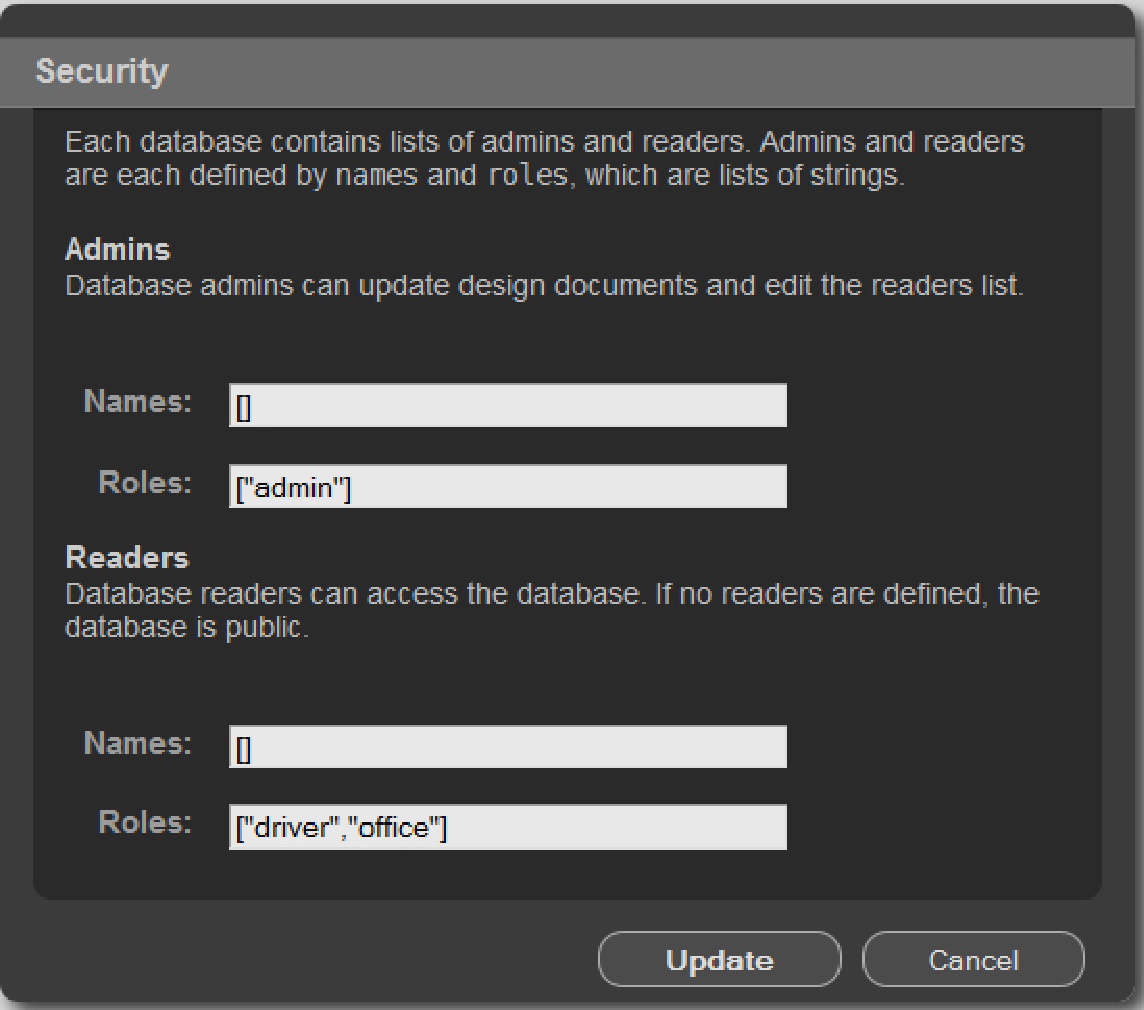
\includegraphics[width=0.8\textwidth]{files/pdf/security.pdf}
	\caption{Admins \& Readers}
	\label{fig:security}
\end{figure}

Auf einer Datenbank können in CouchDB Admins und Readers definiert werden. 
\begin{description}
\item[Admin] Ein Admin hat sämtliche Rechte auf der Datenbank. Er kann die zudem die Datenbank löschen, Designdokumente verändern oder Benutzerrechte ändern.
\item[Reader] Ein Reader hat lesenden und schreibenden Zugriff auf alle Dokumente bis auf die Designdokumente.
\end{description}

\noindent Ein Benutzer kann über 2 verschiedene Arten einer Gruppe zugeordnet werden:
 \begin{itemize}
\item Names: Ein CouchDB-Benutzer muss einen eindeutigen Namen im Format "`org.couchdb.user:[username]"' haben. Die Benutzer werden in einer seperaten Datenbank mit dem Namen "`\_users"' definiert. Wenn der Benutzer dieser Liste (Array aus Strings) hinzugefügt wird, dann besitzt er die entsprechenden Rechte.
\item Roles: Ein Benutzer kann verschiedene Rollen besitzen. Wenn eine seiner Rollen in dieser Liste aufgeführt wird, hat er die entsprechenden Rechte. 
\end{itemize}

\subsubsection{Rollen in Roadrunner}

Einem Benutzer können keine bis mehrere Rollen zugewiesen werden. Bei jeder Veränderung von Dokumenten auf dem Backendsystem wird von CouchDB eine Benutzerauthentifizierung durchgeführt. Bei dieser Benutzerauthentifizierung wird das Zugriffsrecht auf die Datenbank überprüft und zudem eine Validierung durchgeführt. Bei der Validierung werden alle definierten Validierungsmethoden aufgerufen. Nur wenn alle Validierungen gültig sind wird die gewünschte Änderung an den Dokumenten durchgeführt.
\newline \newline \noindent
Im Projekt Roadrunner wurden 3 verschiedenen Rollen definiert:
\begin{description}
\item[Admin] Ein Admin hat sämtliche Rechte auf der Datenbank. Diese Rollen ist ausschließlich für Administratoren vorgesehen.
\item[Office] Ein Benutzer der Gruppe Office arbeitet mit dem Backendsystem von Roadrunner. Dieser Benutzer arbeitet über die Webapplikation mit Roadrunner.
\item[Driver] Ein Benutzer der Gruppe Driver ist ein Fahrer. Er arbeitet auf dem Androidsystem mit Roadrunner. Auf dem Androidsystem arbeitet er als Admin mit der Datenbank. Eine Einschränkung der Benutzerrechte auf dem Androidsystem ist nicht nötig da die Benutzerauthentifizierung bei der Replizierung der Daten von dem Androidsystem auf das Backendsystem durchgeführt wird. Ein Fahrer kann nur Daten replizieren für die er die entsprechenden Rechte besitzt.
\end{description}

\noindent In den Validierungsmethoden werden die entpsrechenden Rechtevalidierungen durchgeführt. In Tabelle \ref{tab:rechte} sind die Berechtigungen aufgelistet. Ein + bedeutet, dass der Benutzer das Recht besitzt.

\begin{table}
\begin{tabular}{lccc}
	& Driver & Office & Admin \\
	Benutzerrechte ändern & - & - & + \\
	Designdokumente ändern & - & - & + \\
	Logeinträge anlegen & + & + & + \\
	Logeinträge ändern & - & - & + \\
	Logeinträge löschen & - & - & + \\
	Andere Dokumente anlegen & - & + & + \\
	Andere Dokumente ändern & - & + & + \\
	Andere Dokumente löschen & - & + & +
\end{tabular}
\caption{Benutzerrechte}
\label{tab:rechte}
\end{table}


\clearpage
\section{Wirtschaftliche Betrachtung}
\label{sec:business}

TODO

\clearpage
\section{Projektentwicklung}
\label{sec:development}

\subsection{Usecases}

\subsubsection{Login}

Ein Fahrer hat im System einen Benutzer. Durch Benutzername und Passwort kann sich der Fahrer auf dem Android-System einloggen. Als Authentifizierungssystem zum Server werden dabei CouchDB-User verwendet. Details zum Authentifizierungssystem sind unter Abschnitt \ref{security}.

Nach dem Einloggen kann der Fahrer sein Fahrzeug wählen. Das Auswählen des Fahrzeuges ist notwendig, damit das Android-System weiß welche Sensoren auszulesen sind. In Kapitel \ref{sensors} ist beschrieben wie jedes Fahrzeug mit Sensoren ausgestattet wird. 

In Abbildung \ref{fig:login} ist ersichtlich wie der Loginvorgang durchgeführt wird. Nach dem Loginvorgang versucht das System eine Anfrage für neue Daten an den Server zu senden.  Bei einer aktiven Serververbindung werden die Benutzerdaten und das gewählte Fahrzeug an den Server gesendet. Nach einer Authentifizierung des Benutzers wird ermittelt ob für das gewählte Fahrzeug neue Daten bezüglich der Sensoren vorhanden sind. Sind neue Daten vorhanden werden diese per Datenbankreplikation an das mobile Gerät gesendet.

Bei der Replikation werden Container-Dokumente übertragen. In diesen Dokumenten sind die Informationen gespeichert, welche Sensoren auf dem jeweiligen Fahrzeug vorhanden sind und wie diese anzusprechen sind.

\begin{figure}
	\centering
		\includegraphics[width=\textwidth]{files/pdf/Login.pdf}
	\caption{Loginvorgang}
	\label{fig:login}
\end{figure}


\begin{itemize}
  \item Wareneingang
  	\subitem registriert Pakete im System
  	\subitem klebt QR-Code auf Pakete

	\item Logister plant und erstellt Lieferungen (neue Auftragsnummer wird
	generiert) \subitem wählt Pakete aus (können mit Sensoren bestückt sein)
		\subitem wählt Fahrer aus 
		\subitem wählt Transportmittel (können mit Sensoren bestückt sein) für
		Lieferungen aus
		\subitem trägt Zielort und Auftraggeber ein
  	
  \item Transporteur
  	\subitem holt oder hat Device mit Roadrunner App
  	\subitem loggt sich im Roadrunner System ein
  		\subsubitem mit Benutzerdaten wird sein/e aktuelle/r Auftrag/Lieferung aufs
  		Device synchronisiert ODER 
  		\subsubitem scannt Pakete und lädt sie in das vom Logistiker ausgwählte
  		Transportmittel
\end{itemize}

\paragraph{Daten-Synchronisierung}
	\textbf{Vorbedingungen: }
	\begin{itemize}
	  \item Transporteur hat sich in der System-App eingeloggt
	\end{itemize}
	
	Die Daten-Synchronisierung oder Replizierung wird durch das Einloggen im
	System angestoßen. Das mobile Gerät erhält folgende Information:
	\begin{itemize}
	  \item Adressen der Sensoren, die das Gerät überwachen sollte
	  \item alle Produkte, Pakete der aktuellen Lieferung, sowie Zielort, etc.
	  \item Überwachungs-Thresholds der Pakete
	\end{itemize}
\par

\subsection{Iteration 1}

\subsubsection{Ziele}

\begin{itemize}
  \item Produkte können erzeugt werden.
  \item Produkte können eingelagert werden.
  \item Produkte können ausgelagert werden.
\end{itemize}

\subsubsection{UML}

\begin{figure}
	\centering
		\includegraphics[width=\textwidth]{files/pdf/Iteration1.pdf}
	\caption{Iteration 1}
	\label{fig:Iteration1}
\end{figure}


\clearpage
\section{Projektunterstützende Werkzeuge und Hilfsmittel}
\label{sec:tools}

In diesem Projekt wurden mehrere projektunterstützende Werkzeuge verwendet.
	Durch den sehr agilen Entwicklungsprozess (siehe Kapitel~\ref{sec:development})
	wurden vor allem auf eine entsprechende Versionskontrolle sowie ein
	Continuous-Integration-Server zur Überwachung des jeweiligen Entwicklungsstands
	geachtet. Diese beiden Systeme sind in den nachfolgenden Abschnitten erläutert.

\subsection{Versionskontrollsystem GIT mit github.com}
\label{subsec:git}

Git ist ein verteiltes Revisions-Kontroll-System mit einem Schwerpunkt auf
	Geschwindigkeit. Git wurde ursprünglich entworfen und
	entwickelt von Linus Torvalds für Linux-Kernel-Entwicklung \cite{Torvalds07}.
	Jedes Git-Arbeitsverzeichnis ist ein vollwertiges \emph{Repository} mit
	kompletter Historie und vollständige Überarbeitung Tracking-Fähigkeiten,
	nicht abhängig von Netzwerkzugang oder einen zentralen Server. Git aktuellen
	Software-Wartung wird durch Junio Hamano betreut. Git ist freie Software unter
	den Bedingungen der GNU General Public License Version 2 verteilt.
	
In diesem Projekt wurde Git für alle Teile des Projekts eingesetzt. Es wurde sowohl
	die CouchDB Applikation, die Android Applikation, die Webapplikation sowie die
	Dokumentation via Git verwaltetet und alle Projektmitglieder konnten in alle
	Teile einsehen sowie mitarbeiten.
	
Um Git auch Online zu synchronisieren, wurde in diesem Projekt
	gihub.com\footnote{vgl. \url{http://github.com}} verwendet. Via github ist es
	möglich, zusätzliche projektunterstützende Werkzeuge (wie z.B. Issue-Tracking,
	Wiki, etc.) zu verwenden.

\subsection{Continious Integration mit Jenkins}
\label{subsec:ci}

Jenkins, früher bekannt als Hudson bekannt, ist eine Open-Source-Continuous
	Integration (CI)-Tool, welches in Java geschrieben ist. Jenkins bietet
	kontinuierliche Integrations-Services für Software-Entwicklung an. Vor
	allem in der Programmiersprache Java. Es ist ein server-basiertes System
	mit einem Servlet-Container wie Apache Tomcat. Es unterstützt SCM-Tools
	einschließlich CVS, Subversion, Git und Clearcase und Apache Ant und Apache
	Maven basierende Projekte, sowie beliebige Shell-Skripte und
	Windows-Batch-Befehle auszuführen. Jenkins ist freie Software und wird
	unter der MIT-Lizenz veröffentlicht.
	
In diesem Projekt wurde sowohl die Android Applikation (Java) sowie die
	Webapplikation automatisiert via Jenkins getestet. Bei jedem neuen
	Commit, welcher zu github synchronisiert wurde, wird automatisiert
	ein Checkout von Jenkins in ein neues Verzeichnis erstellt. Danach
	wird das jeweilige Ant-Build-Script $build.xml$ ausgeführt und die
	Software kompiliert. Anschließend werden die definierten
	Analysewerkzeuge mit einer jeweiligen Konfiguration ausgeführt.
	
Bei der Android Applikation wurden JUnit\footnote{vgl.
	\url{http://www.junit.org/}} Tests ausgeführt.
	
Bei der Webapplikation wurden PHPUnit\footnote{vgl.
	\url{http://www.phpunit.de/}}, PHP-Check-Style, PHP-Mess-Detector sowie
	PHP-Copy-Paste-Detector verwendet um die Qualität zu überprüfen.
	



\clearpage
\section{Zusammenfassung}
\label{sec:fazit}

TODO


%______________________________________________________________________
\cleardoublepage
\pagenumbering{Roman}

\begin{thebibliography}{99}
\addcontentsline{toc}{section}{Literaturverzeichnis}

\bibitem[Gamma 94]{Gamma94}
  E.\ Gamma, R.\ Helm, R.\ Johnson, J.\ Vlissides:
    Design Patterns: Elements of Reusable Object-Oriented Software.
	MA: Addison-Wesley, 1994.

%    Web-References
%______________________________________________________________________

\hspace{-\leftmargin}{\Large\bfseries Web-Referenzen} % Wüster Hack %-|

\bibitem[Wikipedia 10a]{Wikipedia10a}
  Wikipedia: Node.js
    \url{http://de.wikipedia.org/wiki/Node.js}, besucht am 20.04.2011.

\bibitem[Murphy 09]{Murphy09}
	E.\ Murphy:
	CouchDB in Ubuntu
	\url{http://mail-archives.apache.org/mod_mbox/couchdb-dev/200910.mbox/%3C4AD53996.3090104@canonical.com%3E}, besucht am 16.06.2011.

\end{thebibliography}

\cleardoublepage
\begin{appendix}
\section{Appendix}
\label{sec:appendix}

\subsection{Kommerzielle Temperatursensoren}
	\paragraph{Hygrosens TLOG20-BLUE}
		Das ist \textit{NICHT} unsere Lösung.
		\url{http://shop.hygrosens.com/Messsysteme-acma/
			Messsysteme-fuer-Temperatur/Temperaturmesssysteme/
			Temperaturmesssysteme-BLUETOOTH/
			BLUETOOTH-Temperaturmesssystem-20-Kanaele.html}
			{hygrosens.com/TLOG20-BLUE, Zugriff am 16.04.2011}
	\par
	
	\paragraph{Ampedrf BT11}
		Das ist \textit{NICHT} unsere Lösung.
		\url{http://www.ampedrf.com/modules.htm}
		{BT11 Class1, Zugriff am 16.04.2011}
		\url{http://www.ampedrf.com/datasheets/BT11_Datasheet.pdf}
		{BT11 Datasheet}
	\par 

	\paragraph{\$149 Programmable Universal Key Fob Sensor}
		Wir haben uns für das BlueRadios BR-FOB-SEN-LE4.0 Device  entschieden, weil es
		eine komplette und etablierte Lösung für Temperatur, Beschleunigungs- und
		Licht-Messung ist.
		\url{http://www.blueradios.com/BR-FOB-SEN-LE4.0-S2A.pdf}
		{Blueradios BR-FOB-SEN-LE4, Zugriff am 16.04.2011}
		
		\url{http://www.blueradios.com/hardware_sensors.htm}
		{Blueradios BR-FOB-SEN-LE4}
	\par






	\subsubsection{Datenbankinstanzen}
	Anfallende Daten müssen persistent gespeichert werden. Diese Speicherung wird in eine Datenbank durchgeführt. Genauer betrachtet werden die Daten in einer Instanz einer Datenbank gespeichert. Es gilt zu unterscheiden ob eine Instanz einer Datenbank verwendet wird oder mehrere Instanzen verwendet werden und diese synchron gehalten werden.

	\begin{description}
		\item[Eine Instanz] Bei der Verwendung einer Datenbankinstanz gibt es einen zentralen Datenbankserver. Alle Daten werden von dieser Instanz gelesen und geschrieben. Der Vorteil dabei ist, dass alle gespeicherten Daten auf dieser Instanz sofort zur Verfügung stehen. Der Nachteil ist, dass die Datenbank für alle Clients durchgehend zur Verfügung stehen muss.
		\item[Mehrere Instanzen - Jeder synchronisiert mit jedem] Wenn mehrere Instanzen einer Datenbank verwendet werden gilt es diese synchron zu halten. Dies bedeutet, wenn auf einer Instanz Daten erzeugt werden, müssen diese mit anderen Instanzen synchronisiert werden. Eine Möglichkeit ist, dass jede Instanz mit allen anderen Instanzen synchronisiert wird. Dies wäre eine Lösung, wenn es eine definierte Menge von Instanzen gibt und jede Instanz von jeder Instanz aus erreicht werden kann. Dadurch ergibt sich Fehlertoleranz gegenüber Ausfällen von einzelnen Datenbankinstanzen, da die Daten auf jeder Instanz vorliegen und es keine zentrale Masterinstanz gibt.
		\item [Mehrere Instanzen - Jeder synchronisiert mit der Masterinstanz] Anstatt dass jede Instanz mit jeder anderen Instanz synchronisiert wird kann auch eine zentrale Masterinstanz verwendet werden. Diese zentrale Instanz hält alle Daten und verteilt diese Daten wenn nötig auf andere Instanzen. Diese bedeutet wenn eine Clientinstanz neue Daten generiert hat werden diese zur Masterinstanz gesendet und wenn der Client bestimmte Daten benötigt kann er diese bei der Masterinstanz abholen. Dadurch ergibt sich aber ein zentraler Fehlerpunkt. Wenn die Masterinstanz ausfällt ist keine Datenverteilung mehr möglich. 
	\end{description}

	Da beim Roadrunner-Projekt die Daten auf mobilen Geräten erzeugt werden und diese oft auch offline arbeiten, müssen die Daten auf dem Gerät ebenfalls gespeichert werden. Diese Daten werden auf dem Gerät in einer Datenbankinstanz gespeichert. Da es einem mobilen Gerät nicht möglich ist zu allen anderen mobilen Geräten im System Kontakt aufzunehmen wird eine zentrale Masterinstanz verwendet. Auf ein mobiles Gerät werden nur solche Daten gespeichert, die für die Abwicklung der Lieferaufträge benötigt werden.

	\subsubsection{Datenspeicherung}

	Daten können in einer Datenbank auf unterschiedliche Arten gespeichert werden. Dieser Abschnitt beschreibt die unterschiedlichen Speicherungsarten und beschreibt ob diese für das Projekt Roadrunner verwendet werden können.

	\begin{description}
		\item[Relationale Datenbank] In einer relationalen Datenbank werden Daten in einer Tabelle gespeichert. Tabellen werden über PrimaryKey-ForeignKey-Verknüpfungen miteinander in Verbindung gebracht. Ein Eintrag in eine Tabelle, die auf eine andere Tabelle verweist, kann nur durchgeführt werden wenn der Eintrag auf den verweisen wird in der anderen Tabelle existiert. Somit müssten sehr viele Daten auf die mobilen Geräte verteilt werden. Ein Beispiel: Ein Temperatur-Log-Eintrag gehört zu einem Sensor und zu einem Warengut. Das Warengut befindet sich in einem Transportbehälter und muss somit mit diesem Verknüpft werden. Der Transportbehälter hat ein Fahrzeug. Ein Fahrzeug gehört zu einem Fuhrpark usw. Die Verwendung einer relationalen Datenbank auf einem mobilen Gerät wäre nur möglich wenn unterschiedliche Datenbankschemas für die Instanzen der mobilen Geräte und des Masters verwendet werden. 
		\item[Objektorientierte Datenbank] Die Daten werden direkt als Objekte in die Datenbank gespeichert. Da auf den mobilen Geräten aber Java-Objekte bestehen und auf der Webapplikation PHP-Objekte verwendet werden ist diese Lösung nicht ohne intensiven Programmieraufwand für die Konvertierung möglich.
		\item[Dokumentdatenbank] Die Daten werden als Dokumente in die Datenbank gespeichert. Ein Log-Eintrag ist ein Beispiel solch eines Dokumentes. Dokumente sind für sich unabhängige Datensätze die beliebig in einem System verteilt werden können. Dokumente haben Versionsnummern. Anhand der Versionsnummer erkennt eine Datenbankinstanz ob es eine alte Version eines Dokumentes besitzt und kann bei der Masterinstanz eine neue Version des Dokumentes abholen.
	\end{description}

	Bei Roadrunner wird eine verteilte Dokumentdatenbank verwendet. Die verwendete Datenbank verwendet als Dokumentstruktur JSON. Für JSON gibt es eine hohe Integration in Java und PHP und ist somit eine einfach zu verwendende Datenstruktur.

	\subsubsection{Datenverteilung}

	Daten können auf unterschiedliche Arten im System verteilt werden. Eine Möglichkeit wäre die Daten aus der mobilen Datenbankinstanz in die Applikation zu lesen und das Senden der Daten an die Masterinstanz über die Applikation durchzuführen. Eine andere Möglichkeit ist es, die Datenbanksynchronisierung direkt von den Datenbanken durchführen zu lassen. 

	Bei der verwendeten Datenbank im Roadrunner-Projekt wird die Synchronisierung der Daten von den Datenbankinstanzen durchgeführt. Diese Synchronisierung nennt sich Replizierung und es kann dabei angegeben werden welche Daten synchronisiert werden sollen.

	\subsubsection{CouchDB}

	Dieser Abschnitt beschreibt wie CouchDB die Anforderungen erfüllt.

	\subsubsection{Alternative Datenbanksysteme}

	Dieser Abschnitt beschreibt die möglichen alternativen Datenbanksysteme (z.B. Cassandra) und warum CouchDB als Datenbanksystem ausgewählt wurde.





	
\end{appendix}



% ende des hauptteils
\fancyhead[R]{} % Keine Kopfzeile mehr oben auf jeder Seite

\end{document}
